\chapter{Konzept, Entwurf und Implementierung}
\label{cha:implementierung}

% Abschnitt: Implementierungsdetails
\section{Implementierungsdetails}
\label{sec:implementierung:implementierungsdetails}

Wir erklären in diesem Kapitel die einzelnen Funktionen unserer Anwendung ausführlicher. Dies wird unterstützt durch Screenshots und den zugehörigen Mockups, die zu Beginn des Projekts erstellt wurden, um dem Kunden seine Vorstellungen visuell präsentieren zu können.

%Bildervorlage
\begin{figure}[h]
    \centering
    \begin{minipage}{0.49\textwidth}
        \centering
        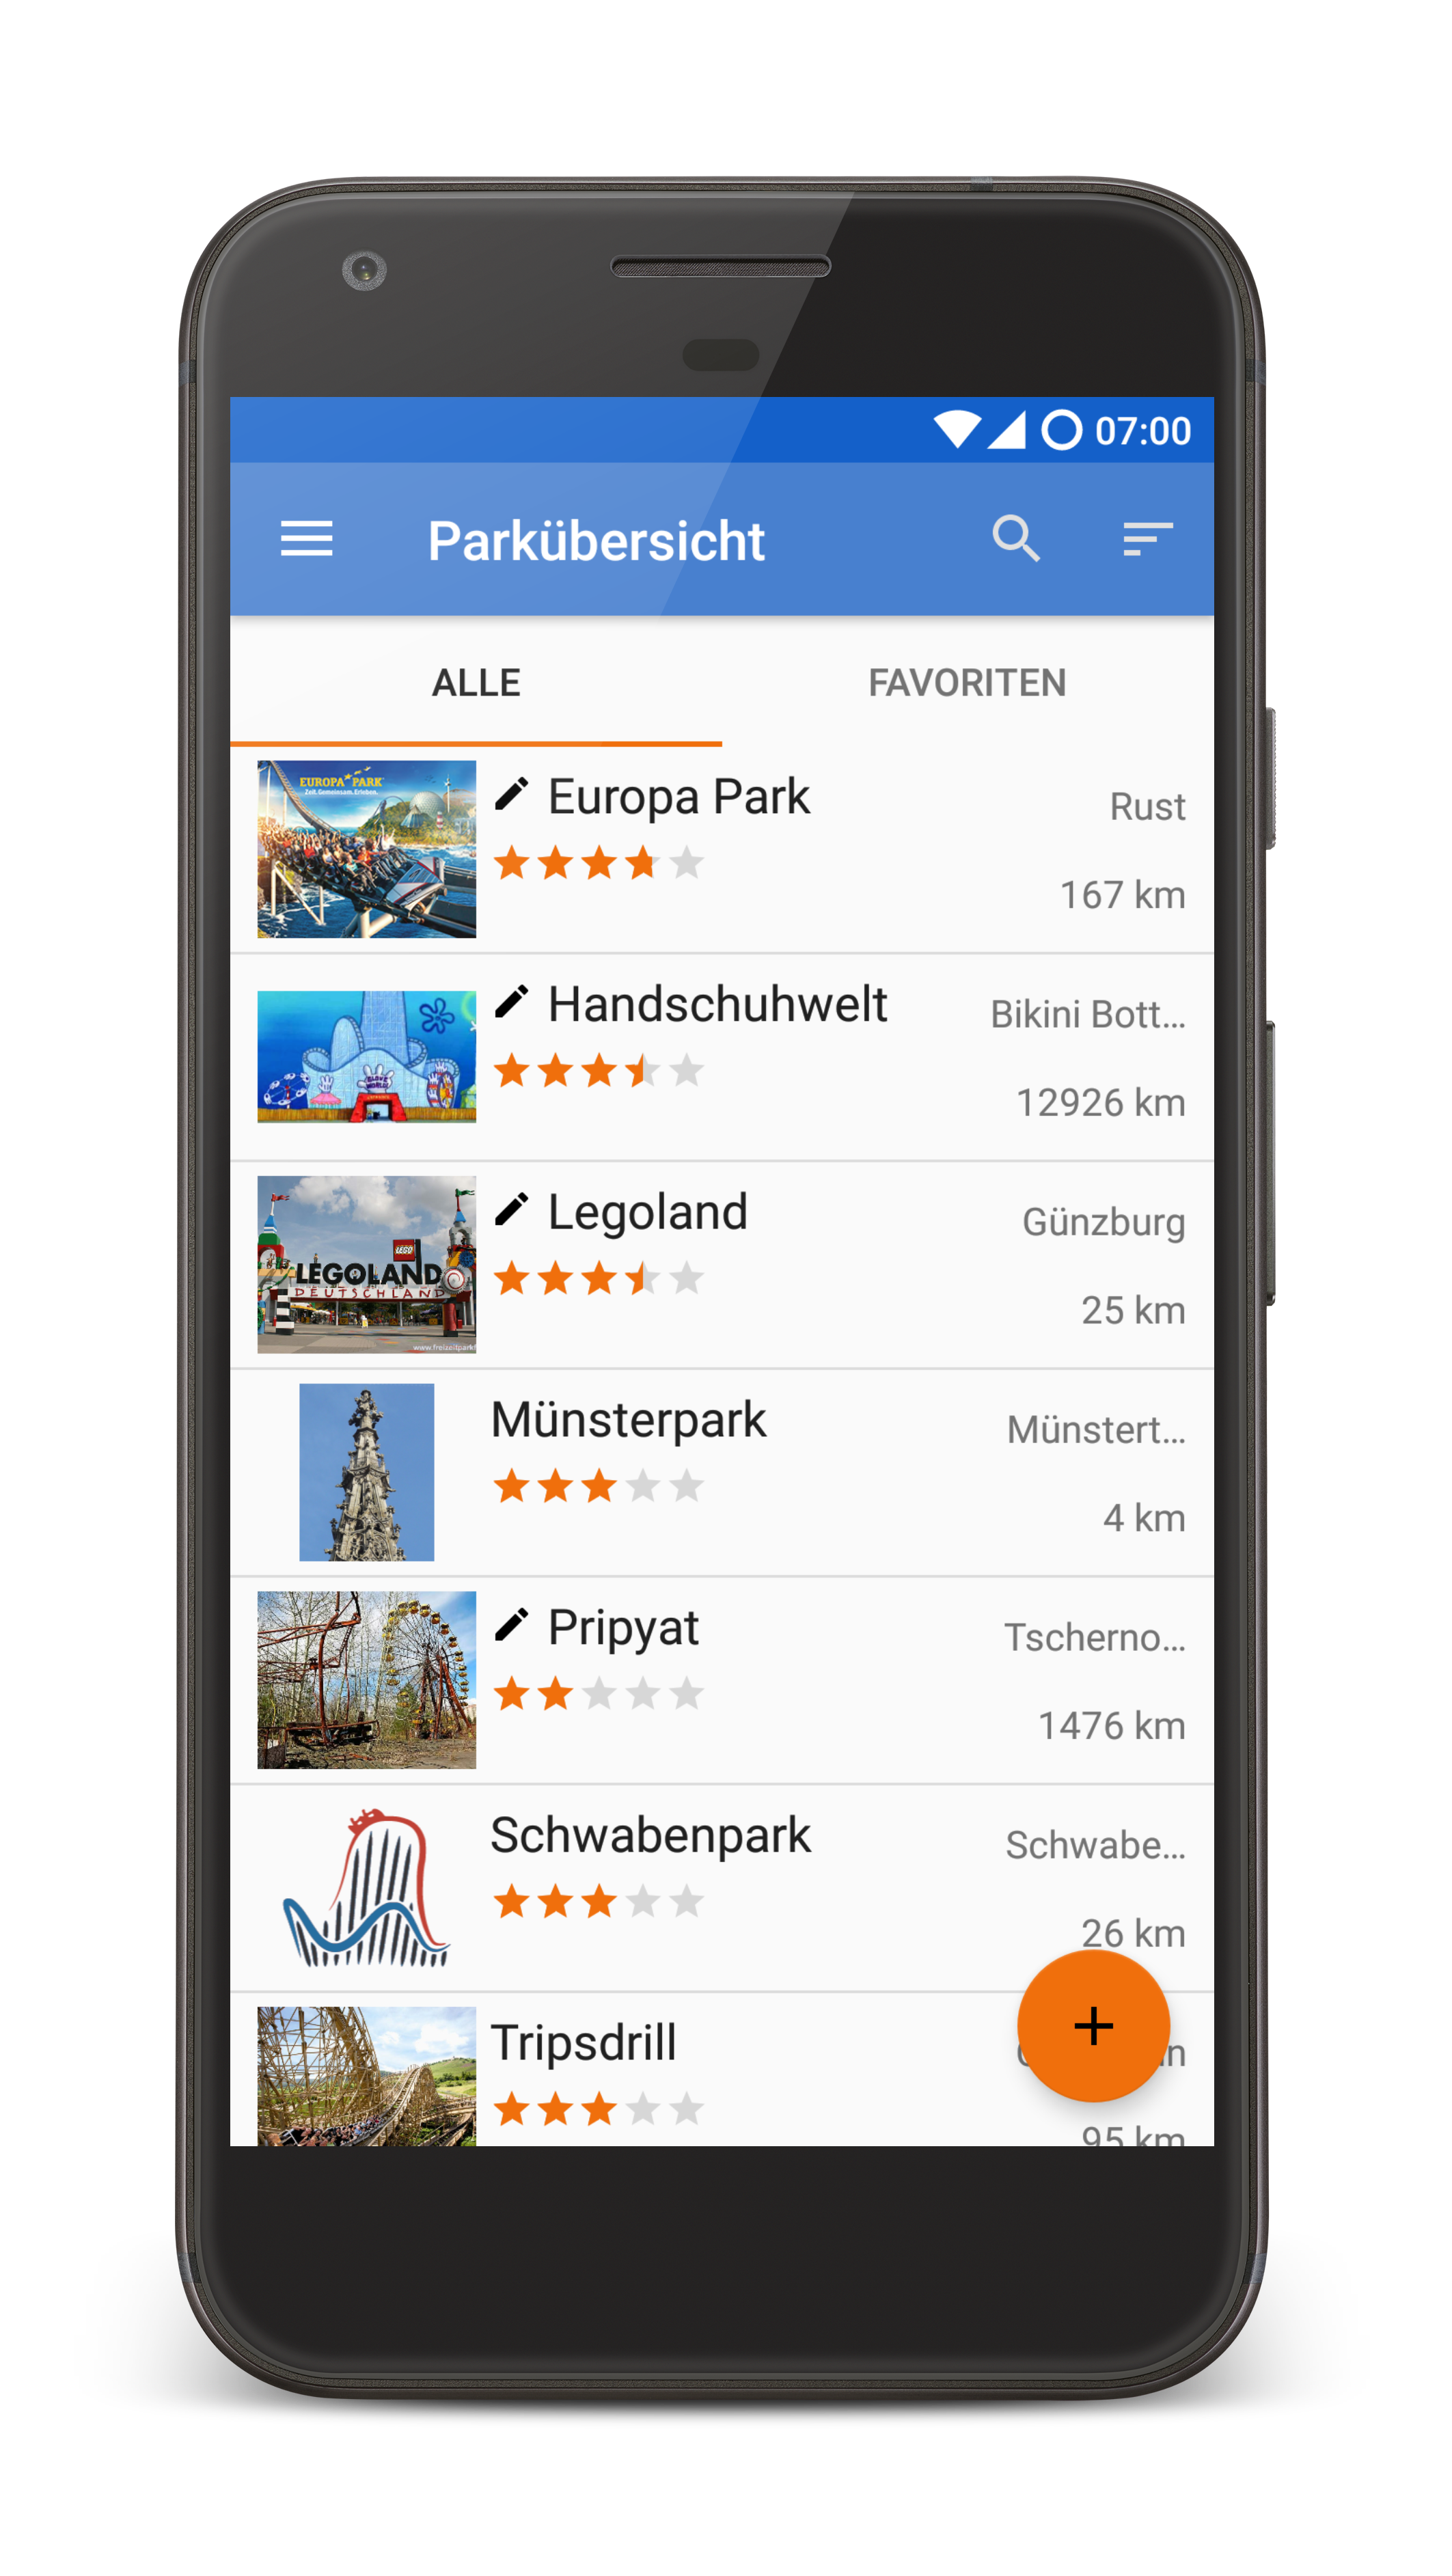
\includegraphics[width=0.4\textwidth]{img/screenshots/ss_parkuebersicht.png}
        \caption{Parkübersicht}
		\label{figure:implementierungparkuebersicht}
    \end{minipage}
    \begin{minipage}{0.49\textwidth}
        \centering
        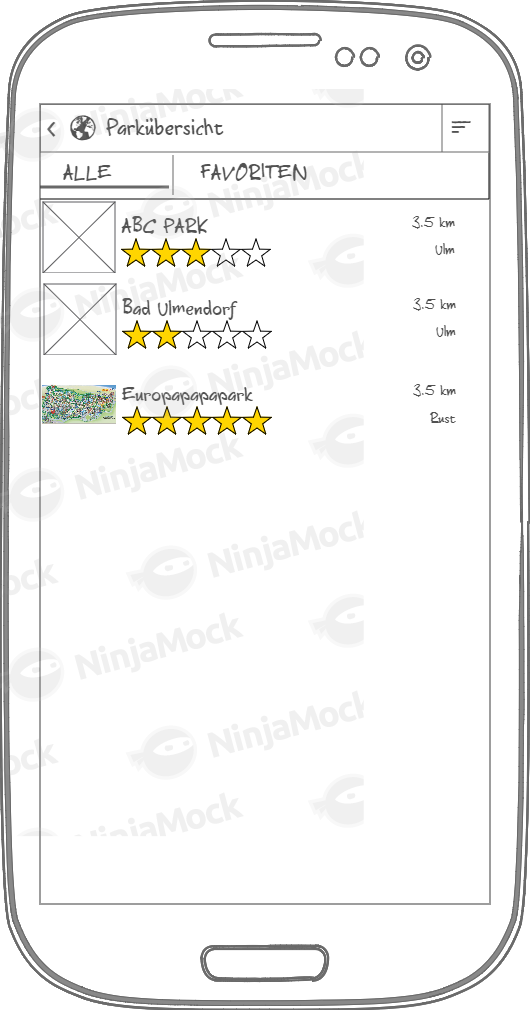
\includegraphics[width=0.4\textwidth]{img/mockups/m_parkuebersicht.png}
        \caption{Mockup Parkübersicht}
    \end{minipage}
\end{figure}



% Abschnitt: Besonderheiten 
\section{Besonderheiten}
\label{sec:implementierung:besonderheiten}

TODO

\subsection{Wartezeit berechung und -darstellung}
\label{sec:implementierung:besonderheiten:wartezeit}

\subsection{Client-Server-Kommunikation mit Azure}
\label{sec:implementierung:besonderheiten:azure}

%Download- und Upload-Verlauf-Modell

\subsection{User-Verwaltung mit Firebase}
\label{sec:implementierung:besonderheiten:firebase}

%Firebase Modell?

\subsection{Parkverwaltung}
\label{sec:implementierung:besonderheiten:parkverwaltung}



% Abschnitt: Architektur
\section{Architektur}
\label{sec:implementierung:architektur}

\subsection{Datenmodell und -speicherung}
\label{sec:implementierung:architektur:datenmodell}

TODO

\subsection{Klassen- und Activity-Architektur}
\label{sec:implementierung:architektur:klassenmodell}

TODO

\subsection{Arbeitsaufteilung}
\label{sec:implementierung:architektur:arbeitsaufteilung}

Während der Implementation wurden die Aufgaben so aufgeteilt, dass jeder aus dem Team immer für eine bestimmte Aufgabe zuständig war und diese durch alle Schichten durch erledigen musste. Bei großen Aufgaben, wie dem Spielablauf, wurden die Aufgabe zudem in kleinere Schritte aufgeteilt. Da die App aus mehreren unabhängigen Bereichen besteht, konnten die Aufgaben gut eingeteilt werden, ohne dass es zu Behinderungen kommt. Wenn gerade keine Arbeit für eine Person angefallen war, beschäftigte diese sich mit Verbesserungen, Testen von Funktionen oder mit der Weiterentwicklung des Designs.

% Abschnitt: Schwierigkeiten während der Implementierung 
\section{Schwierigkeiten während der Implementierung}
\label{sec:implementierung:schwierigkeiten}	

TODO

\begin{itemize} 
\item 1
\item 2
\end{itemize}




